% Generated from figures/generated/ch09-pairing.svg; do not hand edit.
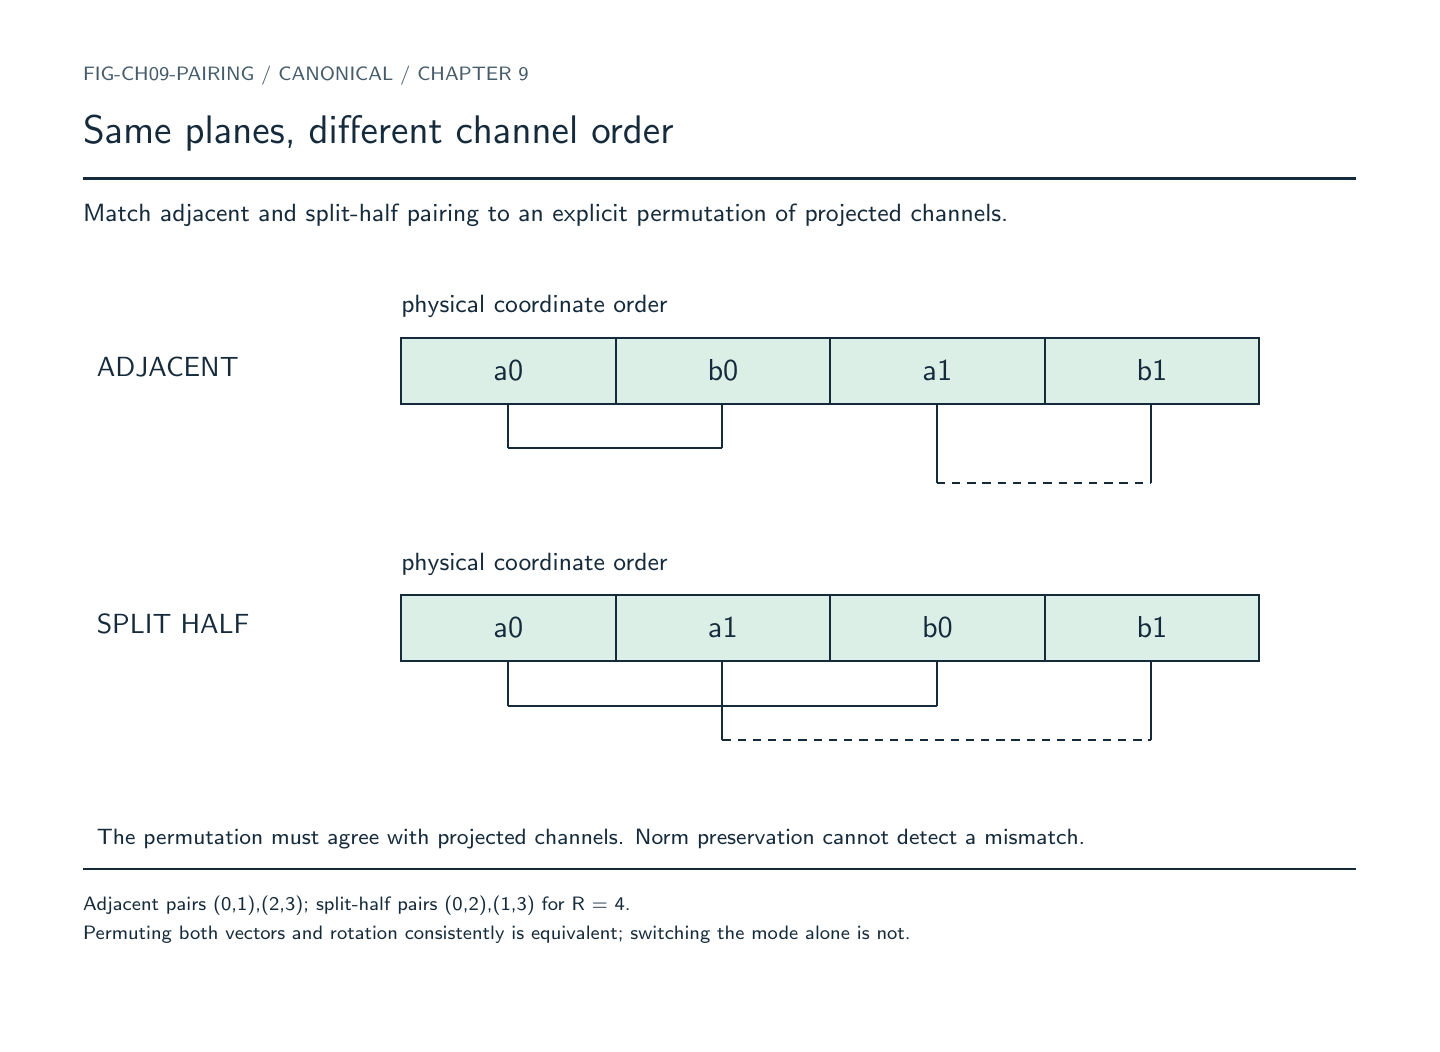
\begin{tikzpicture}[x=.5pt,y=-.5pt]
\path[use as bounding box] (0,0) rectangle (1000,720);
\path[fill=white,draw=none,line width=0.5pt] (0.0,0.0) rectangle (1000.0,720.0);
\node[inner sep=0pt,outer sep=0pt,anchor=base west,text={rgb,255:red,70;green,92;blue,107},font=\sffamily\fontsize{7.0}{8.4}\selectfont] at (40,38) {FIG-CH09-PAIRING  /  CANONICAL / CHAPTER 9};
\node[inner sep=0pt,outer sep=0pt,anchor=base west,text={rgb,255:red,21;green,43;blue,60},font=\sffamily\fontsize{15.0}{18.0}\selectfont] at (40,84) {Same planes, different channel order};
\draw[fill=none,draw={rgb,255:red,21;green,43;blue,60},line width=0.75pt] (40,109) -- (960,109);
\node[inner sep=0pt,outer sep=0pt,anchor=base west,text={rgb,255:red,21;green,43;blue,60},font=\sffamily\fontsize{9.5}{11.4}\selectfont] at (40,140) {Match adjacent and split-half pairing to an explicit permutation of projected channels.};
\node[inner sep=0pt,outer sep=0pt,anchor=base west,text={rgb,255:red,21;green,43;blue,60},font=\sffamily\fontsize{10.0}{12.0}\selectfont] at (50,252) {ADJACENT};
\path[fill={rgb,255:red,220;green,239;blue,231},draw={rgb,255:red,21;green,43;blue,60},line width=0.7pt] (270.0,224.0) rectangle (425.0,272.0);
\node[inner sep=0pt,outer sep=0pt,anchor=base west,text={rgb,255:red,21;green,43;blue,60},font=\sffamily\fontsize{9.5}{11.4}\selectfont] at (284,253) {};
\node[inner sep=0pt,outer sep=0pt,anchor=base,text={rgb,255:red,21;green,43;blue,60},font=\sffamily\fontsize{10.5}{12.6}\selectfont] at (347.5,255) {a0};
\path[fill={rgb,255:red,220;green,239;blue,231},draw={rgb,255:red,21;green,43;blue,60},line width=0.7pt] (425.0,224.0) rectangle (580.0,272.0);
\node[inner sep=0pt,outer sep=0pt,anchor=base west,text={rgb,255:red,21;green,43;blue,60},font=\sffamily\fontsize{9.5}{11.4}\selectfont] at (439,253) {};
\node[inner sep=0pt,outer sep=0pt,anchor=base,text={rgb,255:red,21;green,43;blue,60},font=\sffamily\fontsize{10.5}{12.6}\selectfont] at (502.5,255) {b0};
\path[fill={rgb,255:red,220;green,239;blue,231},draw={rgb,255:red,21;green,43;blue,60},line width=0.7pt] (580.0,224.0) rectangle (735.0,272.0);
\node[inner sep=0pt,outer sep=0pt,anchor=base west,text={rgb,255:red,21;green,43;blue,60},font=\sffamily\fontsize{9.5}{11.4}\selectfont] at (594,253) {};
\node[inner sep=0pt,outer sep=0pt,anchor=base,text={rgb,255:red,21;green,43;blue,60},font=\sffamily\fontsize{10.5}{12.6}\selectfont] at (657.5,255) {a1};
\path[fill={rgb,255:red,220;green,239;blue,231},draw={rgb,255:red,21;green,43;blue,60},line width=0.7pt] (735.0,224.0) rectangle (890.0,272.0);
\node[inner sep=0pt,outer sep=0pt,anchor=base west,text={rgb,255:red,21;green,43;blue,60},font=\sffamily\fontsize{9.5}{11.4}\selectfont] at (749,253) {};
\node[inner sep=0pt,outer sep=0pt,anchor=base,text={rgb,255:red,21;green,43;blue,60},font=\sffamily\fontsize{10.5}{12.6}\selectfont] at (812.5,255) {b1};
\draw[fill=none,draw={rgb,255:red,21;green,43;blue,60},line width=0.75pt] (347,272) -- (347,304);
\draw[fill=none,draw={rgb,255:red,21;green,43;blue,60},line width=0.75pt] (347,304) -- (502,304);
\draw[fill=none,draw={rgb,255:red,21;green,43;blue,60},line width=0.75pt] (502,304) -- (502,272);
\draw[fill=none,draw={rgb,255:red,21;green,43;blue,60},line width=0.75pt] (657,272) -- (657,329);
\draw[fill=none,draw={rgb,255:red,21;green,43;blue,60},line width=0.75pt,dash pattern=on 3.0pt off 2.5pt] (657,329) -- (812,329);
\draw[fill=none,draw={rgb,255:red,21;green,43;blue,60},line width=0.75pt] (812,329) -- (812,272);
\node[inner sep=0pt,outer sep=0pt,anchor=base west,text={rgb,255:red,21;green,43;blue,60},font=\sffamily\fontsize{9.0}{10.799999999999999}\selectfont] at (270,206) {physical coordinate order};
\node[inner sep=0pt,outer sep=0pt,anchor=base west,text={rgb,255:red,21;green,43;blue,60},font=\sffamily\fontsize{10.0}{12.0}\selectfont] at (50,438) {SPLIT HALF};
\path[fill={rgb,255:red,220;green,239;blue,231},draw={rgb,255:red,21;green,43;blue,60},line width=0.7pt] (270.0,410.0) rectangle (425.0,458.0);
\node[inner sep=0pt,outer sep=0pt,anchor=base west,text={rgb,255:red,21;green,43;blue,60},font=\sffamily\fontsize{9.5}{11.4}\selectfont] at (284,439) {};
\node[inner sep=0pt,outer sep=0pt,anchor=base,text={rgb,255:red,21;green,43;blue,60},font=\sffamily\fontsize{10.5}{12.6}\selectfont] at (347.5,441) {a0};
\path[fill={rgb,255:red,220;green,239;blue,231},draw={rgb,255:red,21;green,43;blue,60},line width=0.7pt] (425.0,410.0) rectangle (580.0,458.0);
\node[inner sep=0pt,outer sep=0pt,anchor=base west,text={rgb,255:red,21;green,43;blue,60},font=\sffamily\fontsize{9.5}{11.4}\selectfont] at (439,439) {};
\node[inner sep=0pt,outer sep=0pt,anchor=base,text={rgb,255:red,21;green,43;blue,60},font=\sffamily\fontsize{10.5}{12.6}\selectfont] at (502.5,441) {a1};
\path[fill={rgb,255:red,220;green,239;blue,231},draw={rgb,255:red,21;green,43;blue,60},line width=0.7pt] (580.0,410.0) rectangle (735.0,458.0);
\node[inner sep=0pt,outer sep=0pt,anchor=base west,text={rgb,255:red,21;green,43;blue,60},font=\sffamily\fontsize{9.5}{11.4}\selectfont] at (594,439) {};
\node[inner sep=0pt,outer sep=0pt,anchor=base,text={rgb,255:red,21;green,43;blue,60},font=\sffamily\fontsize{10.5}{12.6}\selectfont] at (657.5,441) {b0};
\path[fill={rgb,255:red,220;green,239;blue,231},draw={rgb,255:red,21;green,43;blue,60},line width=0.7pt] (735.0,410.0) rectangle (890.0,458.0);
\node[inner sep=0pt,outer sep=0pt,anchor=base west,text={rgb,255:red,21;green,43;blue,60},font=\sffamily\fontsize{9.5}{11.4}\selectfont] at (749,439) {};
\node[inner sep=0pt,outer sep=0pt,anchor=base,text={rgb,255:red,21;green,43;blue,60},font=\sffamily\fontsize{10.5}{12.6}\selectfont] at (812.5,441) {b1};
\draw[fill=none,draw={rgb,255:red,21;green,43;blue,60},line width=0.75pt] (347,458) -- (347,490);
\draw[fill=none,draw={rgb,255:red,21;green,43;blue,60},line width=0.75pt] (347,490) -- (657,490);
\draw[fill=none,draw={rgb,255:red,21;green,43;blue,60},line width=0.75pt] (657,490) -- (657,458);
\draw[fill=none,draw={rgb,255:red,21;green,43;blue,60},line width=0.75pt] (502,458) -- (502,515);
\draw[fill=none,draw={rgb,255:red,21;green,43;blue,60},line width=0.75pt,dash pattern=on 3.0pt off 2.5pt] (502,515) -- (812,515);
\draw[fill=none,draw={rgb,255:red,21;green,43;blue,60},line width=0.75pt] (812,515) -- (812,458);
\node[inner sep=0pt,outer sep=0pt,anchor=base west,text={rgb,255:red,21;green,43;blue,60},font=\sffamily\fontsize{9.0}{10.799999999999999}\selectfont] at (270,392) {physical coordinate order};
\node[inner sep=0pt,outer sep=0pt,anchor=base west,text={rgb,255:red,21;green,43;blue,60},font=\sffamily\fontsize{8.5}{10.2}\selectfont] at (50,590) {The permutation must agree with projected channels. Norm preservation cannot detect a mismatch.};
\draw[fill=none,draw={rgb,255:red,21;green,43;blue,60},line width=0.75pt] (40,608) -- (960,608);
\node[inner sep=0pt,outer sep=0pt,anchor=base west,text={rgb,255:red,21;green,43;blue,60},font=\sffamily\fontsize{7.5}{9.0}\selectfont] at (40,638) {Adjacent pairs (0,1),(2,3); split-half pairs (0,2),(1,3) for R = 4.};
\node[inner sep=0pt,outer sep=0pt,anchor=base west,text={rgb,255:red,21;green,43;blue,60},font=\sffamily\fontsize{7.5}{9.0}\selectfont] at (40,659) {Permuting both vectors and rotation consistently is equivalent; switching the mode alone is not.};
\end{tikzpicture}
